\documentclass[11pt]{article}
    %	options include 12pt or 11pt or 10pt
    %	classes include article, report, book, letter, thesis

    \usepackage{amsmath}
    \usepackage{array}
    \setlength\extrarowheight{2pt}
    \usepackage{graphicx}
    \graphicspath{ {/home/shanedrafahl/coms331/hw0} }
    
    \title{HW2}
    \author{Shane Drafahl}
    \date{16 September,2017}

    \begin{document}
    \maketitle

    Recitation: 3:10pm - 4:00pm Gilman 2205 Tue TA: Hugh Potter
    $ \newline \newline $
    1. Prove or disprove the following
    $ \newline \newline $
    (a) $ 5n^{2} - 2n + 26 \in O(n^{2}) $
    $ \newline \newline $
    We will prove this with the def of big oh.
    The def of $ O(n^{2}) $ is there exists positive constants c and $ n_{0} $ such
    that 0 $ \leq $ f(n) $ \leq $ c * g(n) for all $ n_{0} \leq n $. In this case 
    f(n) = $ 5n^{2} - 2n + 26 $ and g(n) = $ n^{2} $. We can divide both sides by
    $ n^{2} $ and we can go from $ 0 \leq 5n^{2} - 2n + 26 \leq c * n^{2} $ to
    $ 0 \leq \frac{24}{n} + 5 \leq c $. $ \frac{24}{n = 1} + 5 $ = 29 and if
    $ f_{1}(n) = \frac{24}{n} + 5 $ then $f_{1}(n + 1) \leq f_{1}(n) $ because as 
    natural number n increases it increases the denominator. C could be 29
    or greater and $ 0 \leq 5n^{2} - 2n + 26 \leq c * n^{2} $ would be true so therefore
    $ 5n^{2} - 2n + 26 \in O(n^{2}) $ because the property is true.
    $ \newline \newline $
    (b) $ \forall_{a} \geq 1 $ : $ a^{n} \in O(n!) $
    $ \newline \newline $
    We will prove this with def of big oh.
    So the given statement is equivalent to  $ 0 \leq a^{n} \leq c * n! $. Using induction
    we can prove it.
    $ \newline \newline $
    Basis: Starting at n = 1 because the performance of an algorithm with n = 0 is irrelevent. 
    $ 0 \ leq a \leq c $ is true because for any a c can be a constant of c  = (a + 1).
    Inductive Hypothesis: Suppoose $ 0 \leq a^{n} \leq c * n! $ is true.
    $ \newline \newline $
    Inductive Step:
    We need to prove $ 0 \leq a^{n + 1} \leq c * n! * (n + 1) $. $ a^{n + 1} $ increases by
    some a multiplied by $ a * a^{n} $ from the IH. While the right side $ c * n! * (n + 1) $ from the
    IH is multiplied by (n + 1) for $ c * n! * (n + 1) $. In this case of a, n increases meaning at some point
    it will increase by more when a $<$ n. So the right side is increasing at a faster rate
    then the left side of the comparison. This means that there is a point where $ n! \leq a^{n} $ for some a 
    for a given range of n. We can just say $ c = a^{n} = n! $ for the n where they equal. So for 
    $ 0 \leq a^{n + 1} \leq c * n! * (n + 1) $ if $ a^{n} > n! $ then the constant c multiplied by 
    $ n! * c $ will be greater than or equal to $ a^{n} $ because c is equal to the the value 
    at which n! overtakes $ a^{n} $ so if for n! n is beyond the point where n! overtakes than it will already
    overtake and be a greater value. The other case is that $ a^{n} \leq n! $ for some n then it wont matter what
    c is because n! will be increasing at a greater rate. So $ 0 \leq a^{n + 1} \leq c * n! * (n + 1) $. $ a^{n + 1} $
    is true and therefore $ \forall_{a} \geq 1 $ : $ a^{n} \in O(n!) $ is true.
    $ \newline \newline $
    (c) $ \forall_{a} \geq $ : $ 2^{n + a} \in O(2^{n}) $
    $ \newline \newline $
    To prove for big oh We must prove for $ 0 \leq 2^{n + a} \leq c * 2^{n} $. 
    We can reduce this to $ 0 \leq 2^{n}2^{a} \leq c * 2^{n} $. Because for whatever a is
    we can say that c = $ 2^{a} $ for this value of a so $ 0 \leq 2^{n}2^{a} \leq 2^{a}2^{n} $.
    So obviously this is true You cannot produce a negative number from the exponents either.
    So therefore $ \forall_{a} \geq $ : $ 2^{n + a} \in O(2^{n}) $ is true for all a and n.
    $ \newline \newline $
    (d) $ \forall_{a} > 1 $ : $ (f(n) \in O(log_{2}n)) => (f(n) \in O(log_{a}n)) $
    $ \newline \newline $
    To prove that this is wrong I will use proof of contradiction. 
    Assuming that $ \forall_{a} > 1 $ : $ (f(n) \in O(log_{2}n)) => (f(n) \in O(log_{a}n)) $
    Then either $ f(n) \leq log_{a}(n) \leq log_{2}(n) $ or 
    $ f(n) \leq log_{2}(n) \leq log_{a}(n) $. 
    For $ f(n) \leq log_{2}(n) \leq log_{a}(n) $ a could equal a number greater than 2 and that would
    be a contradiction $ log_{2}(n) \leq log_{3}(n) $ if n is greater than 1.
    Otherwise $ f(n) \leq log_{1}(n) \leq log_{2}(n) $. For this case if f(n) = $ log_{3}(n) $ 
    then for $ log_{a}(n) $, a would have to be between 3 and 2 and a contradiction because 
    it cannot be all values. So therefore $ \forall_{a} > 1 $ : $ (f(n) \in O(log_{2}n)) => (f(n) \in O(log_{a}n)) $
    is not true.
    $ \newline \newline $
    (e) $ 2^{n} \in O(n^{log^{2}n}) $
    $ \newline \newline $
    To disprove this we will use proof of contradiction we will assume that $ 2^{n} \in O(n^{log^{2}n}) $
    is true so $ 0 \leq 2^{n} \leq c * n^{log(n)^{2}} $. If n = 5 then $ 2^{5} $ = 32, and $ 5^{log(5)^{2}} $ = 2.19527...
    So C would need to be 14.5767 or greater for this case. Since we assume it is true we also 
    assume that there is some C for that multiplied by $ n^{log(n)^{2}} $ that would be greater than
    $ 2^{n} $ for all values of n. We will assume that $ 0 \leq 2^{n} \leq c_{1} * n^{log(n)^{2}} $ is
    true where $ c_{1} $ would not need to be increased because its true for all values of n. If we 
    increase n by 1 then $ 2^{n + 1} = 2^{n} * 2 $ would increase 2 multiplied by $ 2^{n} $.
    On the right side $ (n + 1)^{log(n + 1)^{2}} $. For an increase of 1 for log(n) n would 
    have to be increase by log(n * 10) so log(n + 1) would increase less than 1 from log(n). So 
    $ (n + 1)^{log(n + 1)^{2}} $ would not double in size meaning that C would have to increase but
    by contradiction because we assumed that C was the greatest value it needed to be 
    $ 2^{n} \in O(n^{log^{2}n}) $ is not true.
    $ \newline \newline $
    (f) $ 2^{2^{n + 1}} \in O(2^{2^{n}}) $
    $ \newline \newline $
    To disprove this $ 0 \leq 2^{2^{n + 1}} \leq 2^{2^{n}} * C $ we will use proof by contradiction and
    assume this is true and that C is as larg as it needs to be. If we increase n by 1 we get 
    $ 0 \leq 2^{2^{n} * 4} \leq 2^{2^{n} * 2} * C $. $ 2^{2^{n} * 4} $ increases by more than
    $ 2^{2^{n} * 2} * C $ so C would need to be increased but this is a contradiction so therefore 
    by proof of contradiction $ 2^{2^{n + 1}} \in O(2^{2^{n}}) $ is not true.
    $ \newline \newline $
    2. (a) With respect to the input n, what is the worst-case time complexity of the following algorithm?
    $ \newline \newline $
    First we will find in terms of n how many times the outer loop will go. Its going to start with 1
    and go to $ n^{2} $ so we know the outer loop is $ n^{2} $ time complexity. The inner loop
    Takes the value of j and takes the ceil of it. We know that every time it id dividing by 2 untill it reaches 1.
    We know that then $ \frac{j}{2^{y}} $ where y is the total number of times the iner loop loops.
    This is also aproximate to $ 2^{y} $ = j or $ log_{2}(j) $ = y. So we know that the loop will go
    for $ n^{2} * log_{2}(j) $. We also know that j will reach n so the worst-case time complexity is
    $ O(n^{2}log_{2}(n)) $.
    $ \newline \newline $
    (b) Consider the following method that computes the median of an array of consisting of 
    distinct integers.
    $ \newline \newline $
    The best-case time complexity of the algorithm will be the outer for loop is only called once.
    In order for this to happen the inner for loop needs to increase r to n/2 or (n+1)/2 the first time it
    enters the for loop to loop. So The best case is that the first element in the array a[0]
    is larger than (n+1)/2 or n/2 elements from the array. That way the inner for loop will 
    end exactly when r equals n/2 or (n+1)/2. The inner for loop is going to loop around 
    n times and the outer for loop will loop around once. So the big oh notation is
    $ O(n) $ for best case.
    $ \newline \newline $
    For the worst case time complexity we assume that the outer loop is going to loop over the entire 
    array and the inner loop is also going to loop over the entire array every time and either it will 
    return x on the final loop for exit the algorithm without returning x. To get the worst-time
    complexity we would give it an array where the value that is greater than (n+1)/2 or n/2 elements
    of the array is at a[n-1]. So the outer loop will loop n times and the inner loop will loop n times
    also so the big oh notation is $ O(n^{2}) $.
    $ \newline \newline $
    3. Given an array A containing 0s and 1s, such that all the 0s appear in the array before all
    the 1s. Write an algorithm with worst-case time complexity O(log(n)), which finds the
    smallest index i such that A[i] = 1. Describe your algorithm, and analyze its worst-case time
    complexity.
    $ \newline \newline $
    In general the algorithm the will logarithmically search the array by searching for the middle
    of the algorithm and then depending on if there is a 1 to the right of the center of the algorithm
    it will either search the right side of the array or the left side of the array and then 
    either search the left or right side of those sub-arrays and ect untill the 1 is found. 
    The algorithm is as follows.
    $ \newline \newline $
    $ 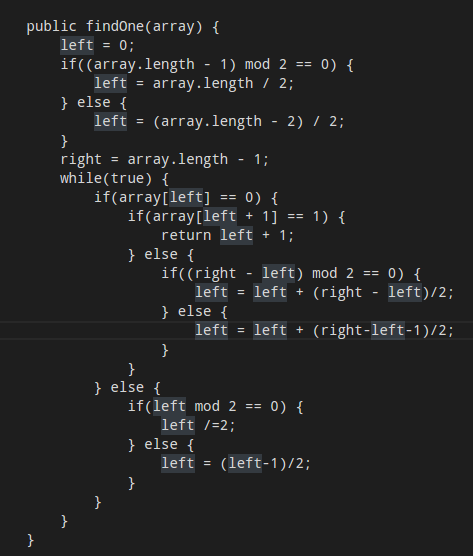
\includegraphics{algo} $
    For the worst time complexity we know that lines between left = 0 and
    right = array.length - 1 are atomic. The while loop will go untill array[left] equals 0 and
    array[left + 1] equals 1. We will say that n is the length of the array given. 
    The variable left is the value of the index in the middle of the array.
    If the 1 is on the right side of the array the algorithm looks in the middle of the right side or 
    vice versa. This means that essentialy it is dividing the array by 2 everytime it searches. The worst
    case is where it divides the array of size n untill the sub array is 1. So 
    $ \frac{n}{2^{y}} $ = 1 where y is some natural number. This is also equal to
    $ 2^{y} = n $ or $ log_{2}(n) = y $. So therefore the time complexity for worst case is 
    $ 7 + log_{2}(n) = O(log(n)) $.
    $ \newline \newline $
    4. Assume that you are given an algorithm named Merge that can merge two sorted integer
    arrays of size n and m to generate a new sorted array of size n + m in O(m + n) time. Your
    task is to use Merge merge k sorted integer arrays each containing n elements, and output a
    single sorted array. Consider the following algorithm for this task. Let A1, A2, ... , Ak be the
    input arrays.
    $ \newline \newline $
    For the given algorithm the for loop will loop around k times.
    the inner for loop takes $ O(m + n) $ time. This means that
    it takes k * (m + n) iterations for the algorithm. If we assume that 
    n is the size of array A and m is the size of some array $ A_{1}, A_{2},...,A_{k} $.
    If the size of array $ k \leq m + n $ then it could take $ k^{2} $ iterations
    as long as the arrays merged are the same size as the total number of arrays or greater than. 
    If k $ < $ m + n then x(m + n) = k. So therefore $ k * (m + n) $ = $ O(k^{2}) $. 
    This is true because $ 0 \leq k * xk \leq c * k^{2} $ where c = x and x * k = (m + n).
    $ \newline \newline $
    5. Consider the following two methods that compute the greatest common divisor of two integers.
    $ \newline \newline $
    (a) gcd took 9797 milliseconds and gcdfast took 0 milliseconds.
    $ \newline \newline $
    (b) gcd took 16225 milliseconds and gcdfast took 0 milliseconds.
    $ \newline \newline $
    (c): Suppose we have inputs a,b where a $ > $ b.
    We then will look at the next recursive step where 
    the inputs will be (b ,c). c = a mod b. One additional step after this
    and the inputs will be (c,d) and d = b mod c. This means 
    that b = xc + d where x is some natural number. We know that
    a $ > $ b. So this means that a $ > $ xc + d. We can get 
    (a + b) $ > $ x(c + d) + b .... (a + b) $ > $ x2(c + d). So 
    for each iteration the value is decreased by half or more.
    For digits a and b that are represented by n digits at least
    each iteration there will be n-1 digits at most for
    the second iteration. The algorithm ends when b equals 0
    so the algorithm goes untill there are no bits left. 
    So therefore the algorithm will be O(n) for n number of 
    bits for a,b.

    \end{document}
